% Options for packages loaded elsewhere
\PassOptionsToPackage{unicode}{hyperref}
\PassOptionsToPackage{hyphens}{url}
\PassOptionsToPackage{dvipsnames,svgnames,x11names}{xcolor}
%
\documentclass[
  letterpaper,
  DIV=11,
  numbers=noendperiod]{scrartcl}

\usepackage{amsmath,amssymb}
\usepackage{iftex}
\ifPDFTeX
  \usepackage[T1]{fontenc}
  \usepackage[utf8]{inputenc}
  \usepackage{textcomp} % provide euro and other symbols
\else % if luatex or xetex
  \usepackage{unicode-math}
  \defaultfontfeatures{Scale=MatchLowercase}
  \defaultfontfeatures[\rmfamily]{Ligatures=TeX,Scale=1}
\fi
\usepackage{lmodern}
\ifPDFTeX\else  
    % xetex/luatex font selection
\fi
% Use upquote if available, for straight quotes in verbatim environments
\IfFileExists{upquote.sty}{\usepackage{upquote}}{}
\IfFileExists{microtype.sty}{% use microtype if available
  \usepackage[]{microtype}
  \UseMicrotypeSet[protrusion]{basicmath} % disable protrusion for tt fonts
}{}
\makeatletter
\@ifundefined{KOMAClassName}{% if non-KOMA class
  \IfFileExists{parskip.sty}{%
    \usepackage{parskip}
  }{% else
    \setlength{\parindent}{0pt}
    \setlength{\parskip}{6pt plus 2pt minus 1pt}}
}{% if KOMA class
  \KOMAoptions{parskip=half}}
\makeatother
\usepackage{xcolor}
\setlength{\emergencystretch}{3em} % prevent overfull lines
\setcounter{secnumdepth}{-\maxdimen} % remove section numbering
% Make \paragraph and \subparagraph free-standing
\ifx\paragraph\undefined\else
  \let\oldparagraph\paragraph
  \renewcommand{\paragraph}[1]{\oldparagraph{#1}\mbox{}}
\fi
\ifx\subparagraph\undefined\else
  \let\oldsubparagraph\subparagraph
  \renewcommand{\subparagraph}[1]{\oldsubparagraph{#1}\mbox{}}
\fi

\usepackage{color}
\usepackage{fancyvrb}
\newcommand{\VerbBar}{|}
\newcommand{\VERB}{\Verb[commandchars=\\\{\}]}
\DefineVerbatimEnvironment{Highlighting}{Verbatim}{commandchars=\\\{\}}
% Add ',fontsize=\small' for more characters per line
\usepackage{framed}
\definecolor{shadecolor}{RGB}{241,243,245}
\newenvironment{Shaded}{\begin{snugshade}}{\end{snugshade}}
\newcommand{\AlertTok}[1]{\textcolor[rgb]{0.68,0.00,0.00}{#1}}
\newcommand{\AnnotationTok}[1]{\textcolor[rgb]{0.37,0.37,0.37}{#1}}
\newcommand{\AttributeTok}[1]{\textcolor[rgb]{0.40,0.45,0.13}{#1}}
\newcommand{\BaseNTok}[1]{\textcolor[rgb]{0.68,0.00,0.00}{#1}}
\newcommand{\BuiltInTok}[1]{\textcolor[rgb]{0.00,0.23,0.31}{#1}}
\newcommand{\CharTok}[1]{\textcolor[rgb]{0.13,0.47,0.30}{#1}}
\newcommand{\CommentTok}[1]{\textcolor[rgb]{0.37,0.37,0.37}{#1}}
\newcommand{\CommentVarTok}[1]{\textcolor[rgb]{0.37,0.37,0.37}{\textit{#1}}}
\newcommand{\ConstantTok}[1]{\textcolor[rgb]{0.56,0.35,0.01}{#1}}
\newcommand{\ControlFlowTok}[1]{\textcolor[rgb]{0.00,0.23,0.31}{#1}}
\newcommand{\DataTypeTok}[1]{\textcolor[rgb]{0.68,0.00,0.00}{#1}}
\newcommand{\DecValTok}[1]{\textcolor[rgb]{0.68,0.00,0.00}{#1}}
\newcommand{\DocumentationTok}[1]{\textcolor[rgb]{0.37,0.37,0.37}{\textit{#1}}}
\newcommand{\ErrorTok}[1]{\textcolor[rgb]{0.68,0.00,0.00}{#1}}
\newcommand{\ExtensionTok}[1]{\textcolor[rgb]{0.00,0.23,0.31}{#1}}
\newcommand{\FloatTok}[1]{\textcolor[rgb]{0.68,0.00,0.00}{#1}}
\newcommand{\FunctionTok}[1]{\textcolor[rgb]{0.28,0.35,0.67}{#1}}
\newcommand{\ImportTok}[1]{\textcolor[rgb]{0.00,0.46,0.62}{#1}}
\newcommand{\InformationTok}[1]{\textcolor[rgb]{0.37,0.37,0.37}{#1}}
\newcommand{\KeywordTok}[1]{\textcolor[rgb]{0.00,0.23,0.31}{#1}}
\newcommand{\NormalTok}[1]{\textcolor[rgb]{0.00,0.23,0.31}{#1}}
\newcommand{\OperatorTok}[1]{\textcolor[rgb]{0.37,0.37,0.37}{#1}}
\newcommand{\OtherTok}[1]{\textcolor[rgb]{0.00,0.23,0.31}{#1}}
\newcommand{\PreprocessorTok}[1]{\textcolor[rgb]{0.68,0.00,0.00}{#1}}
\newcommand{\RegionMarkerTok}[1]{\textcolor[rgb]{0.00,0.23,0.31}{#1}}
\newcommand{\SpecialCharTok}[1]{\textcolor[rgb]{0.37,0.37,0.37}{#1}}
\newcommand{\SpecialStringTok}[1]{\textcolor[rgb]{0.13,0.47,0.30}{#1}}
\newcommand{\StringTok}[1]{\textcolor[rgb]{0.13,0.47,0.30}{#1}}
\newcommand{\VariableTok}[1]{\textcolor[rgb]{0.07,0.07,0.07}{#1}}
\newcommand{\VerbatimStringTok}[1]{\textcolor[rgb]{0.13,0.47,0.30}{#1}}
\newcommand{\WarningTok}[1]{\textcolor[rgb]{0.37,0.37,0.37}{\textit{#1}}}

\providecommand{\tightlist}{%
  \setlength{\itemsep}{0pt}\setlength{\parskip}{0pt}}\usepackage{longtable,booktabs,array}
\usepackage{calc} % for calculating minipage widths
% Correct order of tables after \paragraph or \subparagraph
\usepackage{etoolbox}
\makeatletter
\patchcmd\longtable{\par}{\if@noskipsec\mbox{}\fi\par}{}{}
\makeatother
% Allow footnotes in longtable head/foot
\IfFileExists{footnotehyper.sty}{\usepackage{footnotehyper}}{\usepackage{footnote}}
\makesavenoteenv{longtable}
\usepackage{graphicx}
\makeatletter
\def\maxwidth{\ifdim\Gin@nat@width>\linewidth\linewidth\else\Gin@nat@width\fi}
\def\maxheight{\ifdim\Gin@nat@height>\textheight\textheight\else\Gin@nat@height\fi}
\makeatother
% Scale images if necessary, so that they will not overflow the page
% margins by default, and it is still possible to overwrite the defaults
% using explicit options in \includegraphics[width, height, ...]{}
\setkeys{Gin}{width=\maxwidth,height=\maxheight,keepaspectratio}
% Set default figure placement to htbp
\makeatletter
\def\fps@figure{htbp}
\makeatother

\usepackage{booktabs}
\usepackage{caption}
\usepackage{longtable}
\KOMAoption{captions}{tableheading}
\makeatletter
\makeatother
\makeatletter
\makeatother
\makeatletter
\@ifpackageloaded{caption}{}{\usepackage{caption}}
\AtBeginDocument{%
\ifdefined\contentsname
  \renewcommand*\contentsname{Table of contents}
\else
  \newcommand\contentsname{Table of contents}
\fi
\ifdefined\listfigurename
  \renewcommand*\listfigurename{List of Figures}
\else
  \newcommand\listfigurename{List of Figures}
\fi
\ifdefined\listtablename
  \renewcommand*\listtablename{List of Tables}
\else
  \newcommand\listtablename{List of Tables}
\fi
\ifdefined\figurename
  \renewcommand*\figurename{Figure}
\else
  \newcommand\figurename{Figure}
\fi
\ifdefined\tablename
  \renewcommand*\tablename{Table}
\else
  \newcommand\tablename{Table}
\fi
}
\@ifpackageloaded{float}{}{\usepackage{float}}
\floatstyle{ruled}
\@ifundefined{c@chapter}{\newfloat{codelisting}{h}{lop}}{\newfloat{codelisting}{h}{lop}[chapter]}
\floatname{codelisting}{Listing}
\newcommand*\listoflistings{\listof{codelisting}{List of Listings}}
\makeatother
\makeatletter
\@ifpackageloaded{caption}{}{\usepackage{caption}}
\@ifpackageloaded{subcaption}{}{\usepackage{subcaption}}
\makeatother
\makeatletter
\@ifpackageloaded{tcolorbox}{}{\usepackage[skins,breakable]{tcolorbox}}
\makeatother
\makeatletter
\@ifundefined{shadecolor}{\definecolor{shadecolor}{rgb}{.97, .97, .97}}
\makeatother
\makeatletter
\makeatother
\makeatletter
\makeatother
\ifLuaTeX
  \usepackage{selnolig}  % disable illegal ligatures
\fi
\IfFileExists{bookmark.sty}{\usepackage{bookmark}}{\usepackage{hyperref}}
\IfFileExists{xurl.sty}{\usepackage{xurl}}{} % add URL line breaks if available
\urlstyle{same} % disable monospaced font for URLs
\hypersetup{
  pdftitle={Demographic Health Survey Data in R},
  colorlinks=true,
  linkcolor={blue},
  filecolor={Maroon},
  citecolor={Blue},
  urlcolor={Blue},
  pdfcreator={LaTeX via pandoc}}

\title{{Demographic Health Survey Data in R}}
\usepackage{etoolbox}
\makeatletter
\providecommand{\subtitle}[1]{% add subtitle to \maketitle
  \apptocmd{\@title}{\par {\large #1 \par}}{}{}
}
\makeatother
\subtitle{Pakistan Demographic Health Survey Data}
\author{}
\date{}

\begin{document}
\maketitle
\ifdefined\Shaded\renewenvironment{Shaded}{\begin{tcolorbox}[boxrule=0pt, breakable, borderline west={3pt}{0pt}{shadecolor}, interior hidden, frame hidden, enhanced, sharp corners]}{\end{tcolorbox}}\fi

\renewcommand*\contentsname{Table of contents}
{
\hypersetup{linkcolor=}
\setcounter{tocdepth}{3}
\tableofcontents
}
Prof.Dr. Zahid Asghar, School of Economics,
QAU
\includegraphics{images/zahid.jpg}

\hypertarget{purpose}{%
\subsection{Purpose}\label{purpose}}

Main purpose of this post is to explain how to download and read
\texttt{DHS} data in R, how to create variables, make tables and
cross-tables and run a simple logit regression. I am using in this post
is \texttt{IR} which is the individual (women's) recode file. For more
details about files you can visit \href{dhsprogram.com}{dhs}. USAID main
sponsoring agency of DHS data has recently started using open community
software for \texttt{DHS} data. I am using it for Pakistani data
2017-18. Main outline of this post is as follows:

\begin{enumerate}
\def\labelenumi{\roman{enumi})}
\item
  Reading dhs files in R from STATA (one can do with with SPSS and other
  formats as well)
\item
  Creating new variables , tables, cross-tables, surveydesign and
  regression. I shall mainly use \texttt{tidyverse} package but you can
  use base R if you like.
\end{enumerate}

\hypertarget{install-r-and-rstudio-urduhindi-langues-for-this-heading-only}{%
\subsection{Install R and RStudio (Urdu/Hindi langues for this heading
only)}\label{install-r-and-rstudio-urduhindi-langues-for-this-heading-only}}

Once you have installed R, Rtools (in some cases using Windows) and
RStudio\url{https://youtu.be/ZNBZevfYgo0}, you need to install a
package. A package is like fixing a bulb and you have to do it only
once. Once you have installed relevant package(s), next is to recall it
using \texttt{library()} which is like switching on a button of a bulb.
There is base-R commands but very easy and useful is to learn
\texttt{tidyverse} which consists of many useful packages, we will talk
later on.

As always, the first thing we will do is load the tidyverse.

\emph{Note: If you haven't yet installed the tidyverse, you'll first
have to run the code install.packages(``tidyverse'').} You may get some
warnings when you recall it. Ignore these warnings and go ahead. What
are errors, warnings and messages, you may watch my video
\url{https://youtu.be/SRSNdCZ_QnE}.

\hypertarget{dhs-data-in-r}{%
\subsection{DHS data in R}\label{dhs-data-in-r}}

Please have the dataset downloaded and ready to use. I shall use the IR
file.You can download the model dataset
\href{https://www.dhsprogram.com/data/Model-Datasets.cfm}{here} For the
code below to work, you must save the dataset in the same folder as your
R scripts.

Install and load the packages you need. You only need to install
packages once. After installing a package you can load the package using
the library command.

\hypertarget{load-relevant-packages}{%
\subsubsection{Load relevant packages}\label{load-relevant-packages}}

\begin{Shaded}
\begin{Highlighting}[]
\FunctionTok{library}\NormalTok{(tidyverse) }\CommentTok{\# its an umbrella library containing 9 important and widely used packages of R}
\FunctionTok{library}\NormalTok{(naniar)   }\CommentTok{\# to use replace\_with\_na function}
\FunctionTok{library}\NormalTok{(haven)  }\CommentTok{\# to read STATA/SPSS data}
\FunctionTok{library}\NormalTok{(here)    }\CommentTok{\# to check what is your file path}
\FunctionTok{library}\NormalTok{(labelled) }\CommentTok{\# to get labels of vairables}
\FunctionTok{library}\NormalTok{(pollster)}
\FunctionTok{library}\NormalTok{(gt)  }\CommentTok{\# to get tables}
\FunctionTok{library}\NormalTok{(survey)  }\CommentTok{\# For analysis of complex survey data sets}
\NormalTok{here}\SpecialCharTok{::}\FunctionTok{here}\NormalTok{() }\CommentTok{\# check your path/directory and make sure your data is in this directory}
\end{Highlighting}
\end{Shaded}

\begin{verbatim}
[1] "D:/RepTemplates/pdhsurvey"
\end{verbatim}

\hypertarget{load-data}{%
\subsection{Load data}\label{load-data}}

As I have my data in a folder \texttt{data} , so I am giving a parth
inside here of the relevant folder and then data.

\begin{Shaded}
\begin{Highlighting}[]
\CommentTok{\# open your dataset}
\CommentTok{\#pkir \textless{}{-}  read\_dta(here("data","PKIR71FL.dta"))}
\CommentTok{\# }
\CommentTok{\# save(pkir, file = \textquotesingle{}data/pkir.RData\textquotesingle{}) \#you can save data in R. It will reduce file size and if its correctly save, you can just click on data and it will be uploaded with the command as follows:}

\FunctionTok{load}\NormalTok{(}\StringTok{"D:/RepTemplates/pdhs/data/pkir.RData"}\NormalTok{)}
\end{Highlighting}
\end{Shaded}

\hypertarget{modern-contraceptive-use}{%
\subsection{Modern contraceptive use}\label{modern-contraceptive-use}}

To recode modern contraceptive use into a binary variable, first I check
category labels of \texttt{v313} representing methods used for family
planning.

\begin{Shaded}
\begin{Highlighting}[]
\FunctionTok{print\_labels}\NormalTok{(pkir}\SpecialCharTok{$}\NormalTok{v313)  }\CommentTok{\# print\_labels command for variable labels}
\end{Highlighting}
\end{Shaded}

\begin{verbatim}

Labels:
 value              label
     0          no method
     1   folkloric method
     2 traditional method
     3      modern method
\end{verbatim}

Recode \texttt{v313} as \texttt{1} if female is using modern method and
0 if otherwise. For this I use \texttt{mutate} for creating a new
variable \texttt{modfp}. To create survey weight variables
\texttt{wt}and finally a table of summary statistics is calculated.

\begin{Shaded}
\begin{Highlighting}[]
\CommentTok{\# creating a new categorical variable using mutate and case\_when commands}

\NormalTok{pkir }\OtherTok{\textless{}{-}}\NormalTok{ pkir }\SpecialCharTok{|\textgreater{}}
  \FunctionTok{mutate}\NormalTok{(}\AttributeTok{modfp =}
           \FunctionTok{case\_when}\NormalTok{(v313 }\SpecialCharTok{==} \DecValTok{3} \SpecialCharTok{\textasciitilde{}} \DecValTok{1}\NormalTok{,}
\NormalTok{                     v313 }\SpecialCharTok{\textless{}} \DecValTok{3} \SpecialCharTok{\textasciitilde{}} \DecValTok{0}\NormalTok{ )) }\SpecialCharTok{|\textgreater{}}
  \FunctionTok{set\_value\_labels}\NormalTok{(}\AttributeTok{modfp =} \FunctionTok{c}\NormalTok{(}\AttributeTok{yes =} \DecValTok{1}\NormalTok{, }\AttributeTok{no =} \DecValTok{0}\NormalTok{)) }\SpecialCharTok{|\textgreater{}}
  \FunctionTok{set\_variable\_labels}\NormalTok{(}\AttributeTok{modfp =}\StringTok{"Currently used any modern method"}\NormalTok{)}

\CommentTok{\# creating the sampling weight variable. }
\NormalTok{pkir }\OtherTok{\textless{}{-}}\NormalTok{ pkir }\SpecialCharTok{|\textgreater{}} \FunctionTok{mutate}\NormalTok{(}\AttributeTok{wt=}\NormalTok{v005}\SpecialCharTok{/}\DecValTok{1000000}\NormalTok{)}
\CommentTok{\#pkir$wt \textless{}{-} pkir$v005/1000000}

\CommentTok{\# check with final report Table 7.3}
\FunctionTok{topline}\NormalTok{(pkir, modfp, wt ) }\SpecialCharTok{|\textgreater{}} \FunctionTok{gt}\NormalTok{()}
\end{Highlighting}
\end{Shaded}

\begin{longtable*}{crrrr}
\toprule
Currently used any modern method & Frequency & Percent & Valid Percent & Cumulative Percent \\ 
\midrule
no & 9353.449 & 75.65067 & 75.65067 & 75.65067 \\ 
yes & 3010.551 & 24.34933 & 24.34933 & 100.00000 \\ 
\bottomrule
\end{longtable*}

There are 24\% females who are using modern family planning methods.

\hypertarget{example-2}{%
\subsection{Example 2}\label{example-2}}

Number of ANC visits in 4 categories that match the table in the final
report age of child needed for this indicator. If b19\_01 is not
available in the data use v008 - b3\_01

\begin{Shaded}
\begin{Highlighting}[]
\NormalTok{ pkir }\OtherTok{\textless{}{-}}\NormalTok{ pkir }\SpecialCharTok{|\textgreater{}}
   \FunctionTok{mutate}\NormalTok{(}\AttributeTok{age =}\NormalTok{ b19\_01)}

\NormalTok{pkir }\OtherTok{\textless{}{-}}\NormalTok{ pkir }\SpecialCharTok{|\textgreater{}}
  \FunctionTok{mutate}\NormalTok{(}\AttributeTok{age =}\NormalTok{ v008 }\SpecialCharTok{{-}}\NormalTok{ b3\_01)}


\NormalTok{pkir }\OtherTok{\textless{}{-}}\NormalTok{ pkir }\SpecialCharTok{|\textgreater{}}
  \FunctionTok{mutate}\NormalTok{(}\AttributeTok{ancvisits =}
           \FunctionTok{case\_when}\NormalTok{(}
\NormalTok{             m14\_1 }\SpecialCharTok{==} \DecValTok{0} \SpecialCharTok{\textasciitilde{}} \DecValTok{0}\NormalTok{ ,}
\NormalTok{             m14\_1 }\SpecialCharTok{==} \DecValTok{1} \SpecialCharTok{\textasciitilde{}} \DecValTok{1}\NormalTok{ ,}
\NormalTok{             m14\_1  }\SpecialCharTok{\%in\%} \FunctionTok{c}\NormalTok{(}\DecValTok{2}\NormalTok{,}\DecValTok{3}\NormalTok{)   }\SpecialCharTok{\textasciitilde{}} \DecValTok{2}\NormalTok{ ,}
\NormalTok{             m14\_1}\SpecialCharTok{\textgreater{}=}\DecValTok{4} \SpecialCharTok{\&}\NormalTok{ m14\_1}\SpecialCharTok{\textless{}=}\DecValTok{90}  \SpecialCharTok{\textasciitilde{}} \DecValTok{3}\NormalTok{ ,}
\NormalTok{             m14\_1}\SpecialCharTok{\textgreater{}}\DecValTok{90}  \SpecialCharTok{\textasciitilde{}} \DecValTok{9}\NormalTok{ ,}
\NormalTok{             age}\SpecialCharTok{\textgreater{}=}\DecValTok{60} \SpecialCharTok{\textasciitilde{}} \DecValTok{99}\NormalTok{ )) }\SpecialCharTok{|\textgreater{}}
  \FunctionTok{replace\_with\_na}\NormalTok{(}\AttributeTok{replace =} \FunctionTok{list}\NormalTok{(}\AttributeTok{ancvisits =} \FunctionTok{c}\NormalTok{(}\DecValTok{99}\NormalTok{))) }\SpecialCharTok{|\textgreater{}}
  \FunctionTok{set\_value\_labels}\NormalTok{(}\AttributeTok{ancvisits =} \FunctionTok{c}\NormalTok{(}\AttributeTok{none =} \DecValTok{0}\NormalTok{, }\StringTok{"1"} \OtherTok{=} \DecValTok{1}\NormalTok{, }\StringTok{"2{-}3"}\OtherTok{=}\DecValTok{2}\NormalTok{, }\StringTok{"4+"}\OtherTok{=}\DecValTok{3}\NormalTok{, }\StringTok{"don\textquotesingle{}t know/missing"}\OtherTok{=}\DecValTok{9}\NormalTok{  )) }\SpecialCharTok{|\textgreater{}}
  \FunctionTok{set\_variable\_labels}\NormalTok{(}\AttributeTok{ancvisits =} \StringTok{"Number of ANC visits"}\NormalTok{)}

\CommentTok{\# check with final report Table 9.2}
\FunctionTok{topline}\NormalTok{(pkir, ancvisits, wt ) }\SpecialCharTok{|\textgreater{}} \FunctionTok{gt}\NormalTok{() }\SpecialCharTok{|\textgreater{}} \FunctionTok{fmt\_number}\NormalTok{(}\AttributeTok{decimals =} \DecValTok{2}\NormalTok{)}
\end{Highlighting}
\end{Shaded}

\begin{longtable*}{crrrr}
\toprule
Number of ANC visits & Frequency & Percent & Valid Percent & Cumulative Percent \\ 
\midrule
none & $816.91$ & $6.61$ & $12.17$ & $12.17$ \\ 
1 & $556.75$ & $4.50$ & $8.30$ & $20.47$ \\ 
2-3 & $1,856.84$ & $15.02$ & $27.67$ & $48.14$ \\ 
4+ & $3,452.49$ & $27.92$ & $51.45$ & $99.59$ \\ 
don't know/missing & $27.83$ & $0.23$ & $0.41$ & $100.00$ \\ 
(Missing) & $5,653.18$ & $45.72$ & NA & NA \\ 
\bottomrule
\end{longtable*}

\begin{Shaded}
\begin{Highlighting}[]
\FunctionTok{library}\NormalTok{(gt)}

\FunctionTok{topline}\NormalTok{(pkir, ancvisits, wt ) }\SpecialCharTok{|\textgreater{}} 
  \FunctionTok{gt}\NormalTok{() }\SpecialCharTok{|\textgreater{}} \FunctionTok{fmt\_number}\NormalTok{(}\AttributeTok{decimals =} \DecValTok{2}\NormalTok{)}
\end{Highlighting}
\end{Shaded}

\begin{longtable*}{crrrr}
\toprule
Number of ANC visits & Frequency & Percent & Valid Percent & Cumulative Percent \\ 
\midrule
none & $816.91$ & $6.61$ & $12.17$ & $12.17$ \\ 
1 & $556.75$ & $4.50$ & $8.30$ & $20.47$ \\ 
2-3 & $1,856.84$ & $15.02$ & $27.67$ & $48.14$ \\ 
4+ & $3,452.49$ & $27.92$ & $51.45$ & $99.59$ \\ 
don't know/missing & $27.83$ & $0.23$ & $0.41$ & $100.00$ \\ 
(Missing) & $5,653.18$ & $45.72$ & NA & NA \\ 
\bottomrule
\end{longtable*}

\begin{Shaded}
\begin{Highlighting}[]
\DocumentationTok{\#\#\# Setting the survey design using the svydesign command from the survey package }\AlertTok{\#\#\#}
\CommentTok{\# the survey design will be saved in an object named mysurvey, you can change this name to another name}
\NormalTok{mysurvey}\OtherTok{\textless{}{-}}\FunctionTok{svydesign}\NormalTok{(}\AttributeTok{id=}\NormalTok{pkir}\SpecialCharTok{$}\NormalTok{v021, }\AttributeTok{data=}\NormalTok{pkir, }\AttributeTok{strata=}\NormalTok{pkir}\SpecialCharTok{$}\NormalTok{v022,  }\AttributeTok{weight=}\NormalTok{pkir}\SpecialCharTok{$}\NormalTok{wt, }\AttributeTok{nest=}\NormalTok{T)}
\FunctionTok{options}\NormalTok{(}\AttributeTok{survey.lonely.psu=}\StringTok{"adjust"}\NormalTok{) }

\CommentTok{\# the option (survey.lonely.psu="adjust") is used to adjust for the case if there is single PSU within a stratum }

\CommentTok{\# now that we have set the survey design, we can use the survey package commands. See below for some examples.}
\end{Highlighting}
\end{Shaded}

\begin{Shaded}
\begin{Highlighting}[]
\CommentTok{\# Modern contraceptive use indicator. This indicator was also produced in the RecodingDHSVars.R}
\NormalTok{pkir }\OtherTok{\textless{}{-}}\NormalTok{ pkir }\SpecialCharTok{\%\textgreater{}\%}
  \FunctionTok{mutate}\NormalTok{(}\AttributeTok{modfp =} 
           \FunctionTok{case\_when}\NormalTok{(v313 }\SpecialCharTok{==} \DecValTok{3}\SpecialCharTok{\textasciitilde{}} \DecValTok{1}\NormalTok{,}
\NormalTok{                     v313}\SpecialCharTok{\textless{}}\DecValTok{3}\SpecialCharTok{\textasciitilde{}} \DecValTok{0}\NormalTok{)) }\SpecialCharTok{\%\textgreater{}\%}   
  \FunctionTok{set\_value\_labels}\NormalTok{(}\AttributeTok{modfp =} \FunctionTok{c}\NormalTok{(}\AttributeTok{yes =} \DecValTok{1}\NormalTok{, }\AttributeTok{no =} \DecValTok{0}\NormalTok{)) }\SpecialCharTok{\%\textgreater{}\%}
  \FunctionTok{set\_variable\_labels}\NormalTok{(}\AttributeTok{modfp =}\StringTok{"Currently used any modern method"}\NormalTok{)}

\CommentTok{\# to get frequencies}
\FunctionTok{svytable}\NormalTok{(}\SpecialCharTok{\textasciitilde{}}\NormalTok{modfp, mysurvey)}
\end{Highlighting}
\end{Shaded}

\begin{verbatim}
modfp
       0        1 
9353.449 3010.551 
\end{verbatim}

\begin{Shaded}
\begin{Highlighting}[]
\CommentTok{\# to get proportions}
\FunctionTok{prop.table}\NormalTok{(}\FunctionTok{svytable}\NormalTok{(}\SpecialCharTok{\textasciitilde{}}\NormalTok{modfp, mysurvey))}
\end{Highlighting}
\end{Shaded}

\begin{verbatim}
modfp
        0         1 
0.7565067 0.2434933 
\end{verbatim}

\begin{Shaded}
\begin{Highlighting}[]
\CommentTok{\#you can save the result in an object}
\NormalTok{table1 }\OtherTok{\textless{}{-}} \FunctionTok{prop.table}\NormalTok{(}\FunctionTok{svytable}\NormalTok{(}\SpecialCharTok{\textasciitilde{}}\NormalTok{v106, mysurvey))}

\CommentTok{\#then you can refer to this object later on}
\NormalTok{table1 }
\end{Highlighting}
\end{Shaded}

\begin{verbatim}
v106
        0         1         2         3 
0.4917832 0.1647189 0.2121359 0.1313621 
\end{verbatim}

\begin{Shaded}
\begin{Highlighting}[]
\CommentTok{\#If you want sampling error (SE) and confidence intervals (CI), you can use svyby with by=1 for total}
\FunctionTok{svyby}\NormalTok{(}\SpecialCharTok{\textasciitilde{}}\NormalTok{modfp,}\AttributeTok{by=}\DecValTok{1}\NormalTok{,  }\AttributeTok{design=}\NormalTok{mysurvey, }\AttributeTok{FUN=}\NormalTok{svymean, }\AttributeTok{vartype=}\FunctionTok{c}\NormalTok{(}\StringTok{"se"}\NormalTok{, }\StringTok{"ci"}\NormalTok{))}
\end{Highlighting}
\end{Shaded}

\begin{verbatim}
  by     modfp          se      ci_l      ci_u
1  1 0.2434933 0.006556505 0.2306428 0.2563438
\end{verbatim}

\begin{Shaded}
\begin{Highlighting}[]
\CommentTok{\#if you want to do this for a categorical variable, then you should add as.factor}
\CommentTok{\#below we did not need as.factor since we had a binary variable}
\CommentTok{\#for instance education level, v106, has four categories. You can estimate the SE and cI for each category.}
\FunctionTok{svyby}\NormalTok{(}\SpecialCharTok{\textasciitilde{}}\FunctionTok{as.factor}\NormalTok{(v106),}\AttributeTok{by=}\DecValTok{1}\NormalTok{,  }\AttributeTok{design=}\NormalTok{mysurvey, }\AttributeTok{FUN=}\NormalTok{svymean, }\AttributeTok{vartype=}\FunctionTok{c}\NormalTok{(}\StringTok{"se"}\NormalTok{, }\StringTok{"ci"}\NormalTok{))}
\end{Highlighting}
\end{Shaded}

\begin{verbatim}
  by as.factor(v106)0 as.factor(v106)1 as.factor(v106)2 as.factor(v106)3
1  1        0.4917832        0.1647189        0.2121359        0.1313621
  se.as.factor(v106)0 se.as.factor(v106)1 se.as.factor(v106)2
1          0.01558661         0.006194613          0.01019698
  se.as.factor(v106)3 ci_l.as.factor(v106)0 ci_l.as.factor(v106)1
1          0.00814183              0.461234             0.1525777
  ci_l.as.factor(v106)2 ci_l.as.factor(v106)3 ci_u.as.factor(v106)0
1             0.1921502             0.1154044             0.5223323
  ci_u.as.factor(v106)1 ci_u.as.factor(v106)2 ci_u.as.factor(v106)3
1             0.1768601             0.2321216             0.1473198
\end{verbatim}

\begin{Shaded}
\begin{Highlighting}[]
\CommentTok{\# Crosstabulation of modfp (modern FP use) and place of education (v106)}
\NormalTok{table2 }\OtherTok{\textless{}{-}} \FunctionTok{svyby}\NormalTok{(}\SpecialCharTok{\textasciitilde{}}\NormalTok{modfp, }\AttributeTok{by =} \SpecialCharTok{\textasciitilde{}}\NormalTok{v106, }\AttributeTok{design=}\NormalTok{mysurvey, }\AttributeTok{FUN=}\NormalTok{svymean, }\AttributeTok{vartype=}\FunctionTok{c}\NormalTok{(}\StringTok{"se"}\NormalTok{, }\StringTok{"ci"}\NormalTok{))}

\NormalTok{table2}
\end{Highlighting}
\end{Shaded}

\begin{verbatim}
  v106     modfp          se      ci_l      ci_u
0    0 0.2101258 0.009068765 0.1923513 0.2279002
1    1 0.2744924 0.016388275 0.2423720 0.3066129
2    2 0.2650724 0.012835547 0.2399152 0.2902296
3    3 0.2946932 0.017590575 0.2602163 0.3291701
\end{verbatim}

\hypertarget{chi-square-results}{%
\subsection{chi-square results}\label{chi-square-results}}

\begin{Shaded}
\begin{Highlighting}[]
\FunctionTok{svychisq}\NormalTok{(}\SpecialCharTok{\textasciitilde{}}\NormalTok{modfp}\SpecialCharTok{+}\NormalTok{v106, mysurvey)}

\CommentTok{\# to see how the survey commands are used for regressions, please check the regression R script. }
\CommentTok{\# To do this for several variables at once, you can do the following}

\CommentTok{\# List of variables to crosstabulate with your outcome}
\NormalTok{variables }\OtherTok{\textless{}{-}} \FunctionTok{c}\NormalTok{(}\StringTok{"v013"}\NormalTok{,}\StringTok{"v106"}\NormalTok{, }\StringTok{"v190"}\NormalTok{,}\StringTok{"v025"}\NormalTok{,}\StringTok{"v024"}\NormalTok{) }

\NormalTok{results }\OtherTok{\textless{}{-}} \FunctionTok{list}\NormalTok{()  }\CommentTok{\# Empty list to store the crosstabulation results}

\CommentTok{\# Loop through the variables}
\ControlFlowTok{for}\NormalTok{ (var }\ControlFlowTok{in}\NormalTok{ variables) \{}
  \CommentTok{\# Crosstabulation using svyby}
\NormalTok{  crosstab }\OtherTok{\textless{}{-}} \FunctionTok{svyby}\NormalTok{(}\SpecialCharTok{\textasciitilde{}}\NormalTok{ modfp, }\AttributeTok{by =} \FunctionTok{as.formula}\NormalTok{(}\FunctionTok{paste}\NormalTok{(}\StringTok{"\textasciitilde{}"}\NormalTok{, var)), }\AttributeTok{design =}\NormalTok{ mysurvey, }\AttributeTok{FUN =}\NormalTok{ svymean, }\AttributeTok{vartype =} \FunctionTok{c}\NormalTok{(}\StringTok{"se"}\NormalTok{, }\StringTok{"ci"}\NormalTok{))}
  
\NormalTok{  chi\_square }\OtherTok{\textless{}{-}} \FunctionTok{svychisq}\NormalTok{(}\FunctionTok{as.formula}\NormalTok{(}\FunctionTok{paste}\NormalTok{(}\StringTok{"\textasciitilde{} modfp +"}\NormalTok{, var)), }\AttributeTok{design =}\NormalTok{ mysurvey)}
  
  \CommentTok{\# Store results in list}
\NormalTok{  results[[var]] }\OtherTok{\textless{}{-}} \FunctionTok{list}\NormalTok{(}\AttributeTok{crosstab =}\NormalTok{ crosstab, }\AttributeTok{chi\_square =}\NormalTok{ chi\_square)}
\NormalTok{\}}

\CommentTok{\# Access the crosstabulation results for each variable}
\ControlFlowTok{for}\NormalTok{ (var }\ControlFlowTok{in}\NormalTok{ variables) \{}
  \FunctionTok{print}\NormalTok{(}\FunctionTok{paste}\NormalTok{(}\StringTok{"Crosstabulation for"}\NormalTok{, var))}
  \FunctionTok{print}\NormalTok{(results[[var]])}
\NormalTok{\}}
\end{Highlighting}
\end{Shaded}

\hypertarget{compute-linear-model}{%
\subsection{Compute linear model}\label{compute-linear-model}}

\begin{Shaded}
\begin{Highlighting}[]
\NormalTok{reg1 }\OtherTok{\textless{}{-}} \FunctionTok{svyglm}\NormalTok{(modfp}\SpecialCharTok{\textasciitilde{}}\DecValTok{1}\SpecialCharTok{+}\NormalTok{v025}\SpecialCharTok{+}\FunctionTok{as.factor}\NormalTok{(v013),}
               \AttributeTok{design =}\NormalTok{ mysurvey,}
               \AttributeTok{family =} \FunctionTok{binomial}\NormalTok{(}\AttributeTok{link =} \StringTok{\textquotesingle{}logit\textquotesingle{}}\NormalTok{))}
\end{Highlighting}
\end{Shaded}

\begin{verbatim}
Warning in eval(family$initialize): non-integer #successes in a binomial glm!
\end{verbatim}

\begin{Shaded}
\begin{Highlighting}[]
\FunctionTok{library}\NormalTok{(broom)}
\end{Highlighting}
\end{Shaded}

\begin{verbatim}
Warning: package 'broom' was built under R version 4.3.1
\end{verbatim}

\begin{Shaded}
\begin{Highlighting}[]
\FunctionTok{tidy}\NormalTok{(reg1)}
\end{Highlighting}
\end{Shaded}

\begin{verbatim}
# A tibble: 8 x 5
  term             estimate std.error statistic  p.value
  <chr>               <dbl>     <dbl>     <dbl>    <dbl>
1 (Intercept)        -2.37     0.226     -10.5  4.43e-23
2 v025               -0.235    0.0685     -3.43 6.60e- 4
3 as.factor(v013)2    0.865    0.211       4.10 4.88e- 5
4 as.factor(v013)3    1.40     0.216       6.45 2.96e-10
5 as.factor(v013)4    1.87     0.214       8.74 4.96e-17
6 as.factor(v013)5    1.96     0.212       9.23 1.12e-18
7 as.factor(v013)6    2.08     0.222       9.33 5.33e-19
8 as.factor(v013)7    1.64     0.227       7.26 1.81e-12
\end{verbatim}

\begin{Shaded}
\begin{Highlighting}[]
\CommentTok{\# unadjusted with place of residence }
\NormalTok{reg1 }\OtherTok{\textless{}{-}} \FunctionTok{svyglm}\NormalTok{(modfp}\SpecialCharTok{\textasciitilde{}} \DecValTok{1}\SpecialCharTok{+}\NormalTok{ v025 , }\AttributeTok{design=}\NormalTok{mysurvey, }\AttributeTok{family=}\FunctionTok{binomial}\NormalTok{(}\AttributeTok{link=}\StringTok{"logit"}\NormalTok{))}
\end{Highlighting}
\end{Shaded}

\begin{verbatim}
Warning in eval(family$initialize): non-integer #successes in a binomial glm!
\end{verbatim}

\begin{Shaded}
\begin{Highlighting}[]
\CommentTok{\# to see the results}
\FunctionTok{summary}\NormalTok{(reg1)}
\end{Highlighting}
\end{Shaded}

\begin{verbatim}

Call:
svyglm(formula = modfp ~ 1 + v025, design = mysurvey, family = binomial(link = "logit"))

Survey design:
svydesign(id = pkir$v021, data = pkir, strata = pkir$v022, weight = pkir$wt, 
    nest = T)

Coefficients:
            Estimate Std. Error t value Pr(>|t|)    
(Intercept) -0.64717    0.10343  -6.257 9.24e-10 ***
v025        -0.30138    0.06782  -4.444 1.12e-05 ***
---
Signif. codes:  0 '***' 0.001 '**' 0.01 '*' 0.05 '.' 0.1 ' ' 1

(Dispersion parameter for binomial family taken to be 1.000081)

Number of Fisher Scoring iterations: 4
\end{verbatim}

\begin{Shaded}
\begin{Highlighting}[]
\CommentTok{\# to get ORs}
\NormalTok{ORreg1 }\OtherTok{\textless{}{-}} \FunctionTok{exp}\NormalTok{(reg1}\SpecialCharTok{$}\NormalTok{coefficients )}
\NormalTok{ORreg1}
\end{Highlighting}
\end{Shaded}

\begin{verbatim}
(Intercept)        v025 
  0.5235268   0.7397958 
\end{verbatim}

\begin{Shaded}
\begin{Highlighting}[]
\CommentTok{\# multivariate models with place of residence (v025), education (v106), and current age (v013)}
\NormalTok{reg2 }\OtherTok{\textless{}{-}} \FunctionTok{svyglm}\NormalTok{(modfp}\SpecialCharTok{\textasciitilde{}} \DecValTok{1}\SpecialCharTok{+}\NormalTok{ v025 }\SpecialCharTok{+} \FunctionTok{as.factor}\NormalTok{(v106) }\SpecialCharTok{+} \FunctionTok{as.factor}\NormalTok{(v013), }\AttributeTok{design=}\NormalTok{mysurvey, }\AttributeTok{family=}\FunctionTok{binomial}\NormalTok{(}\AttributeTok{link=}\StringTok{"logit"}\NormalTok{))}
\end{Highlighting}
\end{Shaded}

\begin{verbatim}
Warning in eval(family$initialize): non-integer #successes in a binomial glm!
\end{verbatim}

\begin{Shaded}
\begin{Highlighting}[]
\FunctionTok{tidy}\NormalTok{(reg2)}
\end{Highlighting}
\end{Shaded}

\begin{verbatim}
# A tibble: 11 x 5
   term             estimate std.error statistic  p.value
   <chr>               <dbl>     <dbl>     <dbl>    <dbl>
 1 (Intercept)        -2.79     0.245     -11.4  1.66e-26
 2 v025               -0.100    0.0697     -1.43 1.52e- 1
 3 as.factor(v106)1    0.389    0.0959      4.06 5.86e- 5
 4 as.factor(v106)2    0.360    0.0852      4.22 2.92e- 5
 5 as.factor(v106)3    0.412    0.105       3.93 9.77e- 5
 6 as.factor(v013)2    0.842    0.210       4.01 7.23e- 5
 7 as.factor(v013)3    1.38     0.216       6.37 4.79e-10
 8 as.factor(v013)4    1.85     0.213       8.69 7.61e-17
 9 as.factor(v013)5    1.97     0.212       9.31 6.24e-19
10 as.factor(v013)6    2.13     0.224       9.50 1.37e-19
11 as.factor(v013)7    1.71     0.229       7.48 4.23e-13
\end{verbatim}

\hypertarget{checking-for-correlations}{%
\subsection{checking for correlations}\label{checking-for-correlations}}

create a subset of data with variables you want to check

\begin{Shaded}
\begin{Highlighting}[]
\NormalTok{cordata }\OtherTok{\textless{}{-}} \FunctionTok{subset}\NormalTok{(pkir, }\AttributeTok{select=}\FunctionTok{c}\NormalTok{(v025, v106, v013 ,v190))}

\NormalTok{mycordata }\OtherTok{\textless{}{-}} \FunctionTok{cor}\NormalTok{(cordata)}
\CommentTok{\# we see that v025 and v190 may be highly correlated}

\CommentTok{\# to produce a correlation plot}
\CommentTok{\#install.packages("corrplot")}
\FunctionTok{library}\NormalTok{(corrplot)}
\end{Highlighting}
\end{Shaded}

\begin{verbatim}
Warning: package 'corrplot' was built under R version 4.3.1
\end{verbatim}

\begin{verbatim}
corrplot 0.92 loaded
\end{verbatim}

\begin{Shaded}
\begin{Highlighting}[]
\FunctionTok{corrplot}\NormalTok{(mycordata)}
\end{Highlighting}
\end{Shaded}

\begin{figure}[H]

{\centering 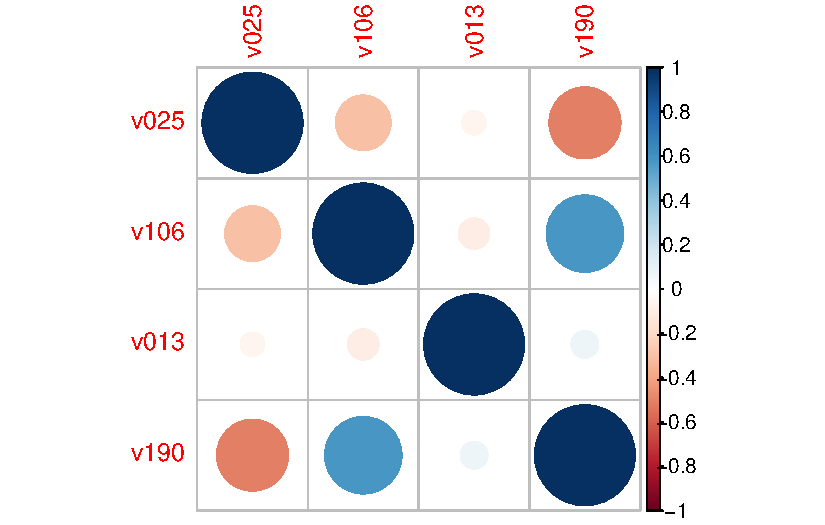
\includegraphics{ir_files/figure-pdf/unnamed-chunk-11-1.pdf}

}

\end{figure}



\end{document}
